\chapter{Knowledge-Based System Integration in a Deep Learning Environment}
\label{chap:kbsintegrationdl}
\textit{The content of this chapter is based on the work \cite{amadoretalontodl}}
\section{Introduction}
\elvitodo{Aquí pos la motivación un poco, limitaciones concretas de esto y por qué}
%Motivaciones de esto: Incrementar capacidad de generalización, reducir número de recursos, aumento de la interpretabilidad del modelo. Restricciones de esto: 

%%%LA MOVIDA DE LA SENSIA EN ESTA VERTIENTE CONCRETA
\section{Existing Limitations of Deep Learning Models}
%Limitaciones y las restricciones estudiadas
\elvitodo{Aquí hay mucha magra en el paper de Frank y las referencias de ese paper}
\section{Ontology-Based Initialization for Knowledge Graph Completion}

This Section provides a case scenario for the introduction of symbolic representations under a deep learning framework, as presented in \cite{amadoretalontodl}. This case scenario focuses on the Knowledge Graph Completion (KGC) task, specifically on its resolution via Knowledge Graph Embedding (KGE) models. As stated in Section ?, KGE models generate vector representations for KGs, subsequently enabling statistical reasoning over the KG. Figure \ref{fig:box_krintodl_base} depicts the baseline design of any KGE model according to the design patterns in \cite{boxologyfrank}. In this scenario, a KG (structured, symbolic) serves as input. Following the standart model generation procedure, the input is divided into three separate subsets: training, validation and test, each containing a different set of facts from the KG. The training set is then fed into a KGE model, which generates a subsymbolic representation for each element of the input. These vector representations can then be used by the same KGE model to infer new potential elements of the KG. 

\begin{figure*}
    \centering
    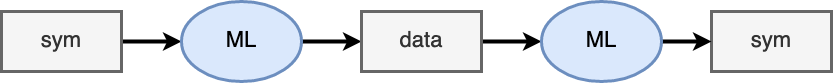
\includegraphics[width=\linewidth]{4_kbsintegrationdl/figures/boxology_krintodl_base.png}
    \caption{Boxology representation of the baseline KGE model}
    \label{fig:box_krintodl_base}
\end{figure*}


While this method provides an efficient solution to the KGC task, two main shortcomings can be identified: (1) they only rely on the information explicitly declared in the input data, thus not considering background, general information that can lead to the inference of general restrictions about the output and (2) they cannot reason over inputs that were not seen by the model during training time.\elvitodo{RELACIONAR ESTO CON LAS LIMITACIONES GENERALES QUE TENEMOS QUE DECLARAR}. Th

\begin{figure*}
    \centering
    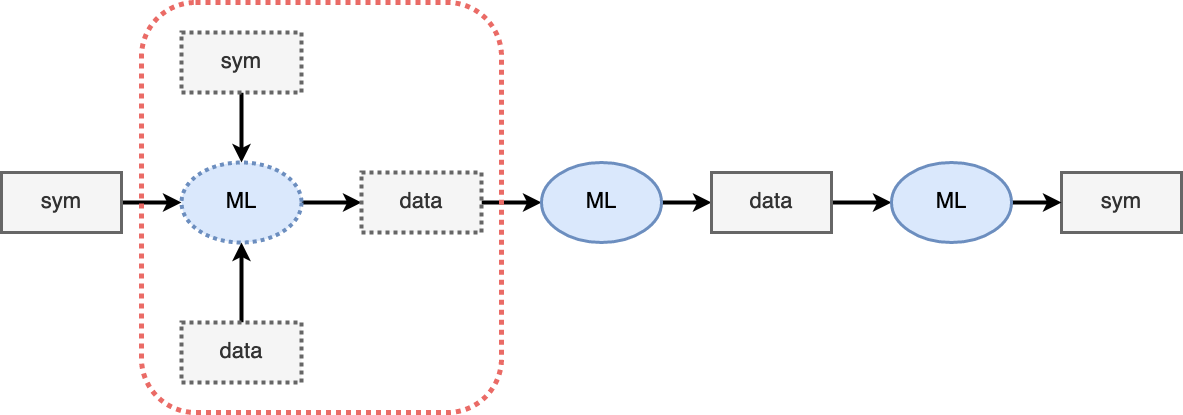
\includegraphics[width=\linewidth]{4_kbsintegrationdl/figures/boxology_krintodl.png}
    \caption{Boxology representation of the proposed hybrid KGE model}
    \label{fig:box_krintodl}
\end{figure*}

\section{Summary}